\chapter{\en{Bandits}}
\label{chap:bandits}
\section{Το πρόβλημα των \en{bandits}}

Το πρόβλημα των ληστών (\en{bandits}), πήρε την ονομασία του από τα μηχανήματα του καζίνο, τους κουλοχέρηδες.
Ο όρος \en{one-arm bandit} προέρχεται από το γεγονός ότι οι κουλοχέρηδες έχουν ένα μοχλό-χέρι και μας "κλέβουν"
τα χρήματα. Η ορολογία στα Ελληνικά δεν είναι ιδιαίτερα καθιερωμένη, οπότε και θα χρησιμοποιήσουμε την Αγγλική.

Το πρόβλημα των \en{bandits} είναι μια απλοποίηση του προβλήματος της Ενισχυτικής Μάθησης.
Στην απλούστερη του μορφή το πρόβλημα δεν είναι προσεταιριστικό, δηλαδή κάθε κατάσταση θεωρείται μοναδικό γεγονός.
Αυτό σημαίνει ότι οι αποφάσεις που κάνει ο πράκτορας στον ένα γύρο δεν επηρεάζουν τις ανταμοιβές και τις επιλογές του
πράκτορα στους επόμενους γύρους. Αυτό είναι το βασικό χαρακτηριστικό τους που κάνει και εμάς να μελετήσουμε
τέτοια προβλήματα, καθώς η χρήση αντίστοιχων τεχνικών επίλυσης μπορεί να μας βοηθήσει να απλοποιήσουμε και το δικό μας πρόβλημα.
Ένα ακόμα σύνηθες χαρακτηριστικό των \en{bandits} είναι ότι ο πράκτορας μπορεί να παρατηρήσει τις ανταμοιβές του σε κάθε γύρο.
Αν δεν μπορεί, τότε το πρόβλημα αυτό λέγεται πρόβλημα \textit{μερικής παρακολούθησης} και δεν είναι κάτι που θα μας απασχολήσει περαιτέρω.

Παρόλο που το πρόβλημα μοιάζει φαινομενικά να είναι πολύ απλούστερο του πλήρους προβλήματος ΕΜ, η επίλυση του δεν είναι τόσο εύκολη.
Σαν παράδειγμα \cite{lattimore2020bandit}, μπορούμε να σκεφτούμε ένα κουλοχέρη που έχει δύο μοχλούς, έναν δεξιό και έναν αριστερό,
τους οποίους τραβώντας τους για 10 γύρους έχουμε τα αποτελέσματα που φαίνονται στον Πίνακα \ref{tab:bandit_example}.

\begin{table}[ht]
    \centering
    \begin{tabularx}{\textwidth}{ccccccccccc}
        \hline
        Γύρος    & 1 & 2  & 3  & 4 & 5 & 6 & 7 & 8 & 9 & 10 \\
        \hline
        Αριστερό & 0 &    & 10 & 0 &   & 0 &   &   &   & 10 \\ \\
        Δεξί     &   & 10 &    &   & 0 &   & 0 & 0 & 0 &    \\
        \hline
    \end{tabularx}
    \caption{Παράδειγμα κουλοχέρη}
    \label{tab:bandit_example}
\end{table}

Αν υποθέσουμε ότι η ανταμοιβή είναι ευρώ, μπορούμε να υπολογίσουμε την μέση ανταμοιβή που έχουμε από κάθε χέρι.
Από αριστερό χέρι έχουμε μέση ανταμοιβή 4€, ενώ από το δεξί έχουμε 2€.Άρα το αριστερό χέρι είναι φαινομενικά καλύτερο.
Aν συνεχίζαμε να παίζουμε και είχαμε ακόμα 10 ακόμα προσπάθειες, ποια θα ήταν η στρατηγική μας από εδώ και πέρα;
Θα χρησιμοποιούσαμε μόνο το αριστερό χέρι για να εκμεταλλευτούμε την πεποίθηση που έχουμε χτίσει, ότι αυτό είναι καλύτερο;
Ή θα χρησιμοποιούσαμε το δεξί χέρι, για να εξερευνήσουμε και να μάθουμε αν η εκτίμηση της ανταμοιβής του είναι σωστή;
Όπως βλέπουμε, το δίλημμα μεταξύ εκμετάλλευσης και εξερεύνησης είναι κεντρικό στα προβλήματα των \en{bandits}.

Η ορολογία που χρησιμοποιούμε στα προβλήματα \en{bandits} είναι η ίδια που χρησιμοποιήσαμε και στα προβλήματα ΕΜ,
με την διαφορά ότι το πλήθος των γύρων που θα παίξει ο πράκτορας ονομάζεται \textbf{ορίζοντας}.
Τα προβλήματα των \en{bandits} είναι προβλήματα που η δυναμική του περιβάλλοντος είναι άγνωστη,
και ο πράκτορας πρέπει να την ανακαλύψει παίζοντας. Το μόνο που γνωρίζει ο πράκτορας για το περιβάλλον είναι ότι βρίσκεται
σε μια οικογένεια περιβαλλόντων $\mathcal{E}$.

Κύρια μετρική της ποιότητας μιας πολιτικής είναι η μετάνοια (\en{regret}), η οποία εκφράζει τη διαφορά μεταξύ των
αναμενόμενων ανταμοιβών μιας πολιτικής $π$ σε $n$ γύρους (η οποία δεν είναι απαραίτητα η πολιτική που ακολούθησε ο πράκτορας),
και των ανταμοιβών που πραγματικά αυτός πήρε σε $n$ γύρους,με βάση την πολιτική που ακολούθησε.
Πολλές φορές είναι χρήσιμο να υπολογίσουμε την μετάνοια και σε σχέση με μια οικογένεια πολιτικών $Π$.
Τότε, η μετάνοια είναι η διαφορά της πολιτικής που ακολούθησε ο πράκτορας σε σχέση με την πολιτική η οποία έχει τις μεγαλύτερες ανταμοιβές
μεταξύ όλων των πολιτικών της οικογένειας $Π$ (με άλλα λόγια την καλύτερη πολιτική). Συνήθως επιλέγουμε την οικογένεια $Π$, ώστε η βέλτιστη πολιτική
για όλη την οικογένεια $\mathcal{E}$ να βρίσκεται μέσα στην οικογένεια πολιτικών $Π$.
Ήδη διαισθητικά καταλαβαίνουμε ότι μεγάλη μετάνοια σημαίνει ότι ο πράκτορας δεν τα πάει καλά,
ενώ μικρή μετάνοια σημαίνει ότι η πολιτική που ακολουθεί είναι κοντά στην βέλτιστη.

Για να μπορέσουμε να λύσουμε το πρόβλημα, συνήθως μειώνουμε τόσο την οικογένεια πρακτόρων, όσο και την οικογένεια των περιβαλλόντων,
ώστε να περιέχει στοιχεία που έχουν συγκεκριμένες επιθυμητές ιδιότητες. Στόχος κάθε φορά είναι να δημιουργήσουμε αλγορίθμους που να
πετυχαίνουν όσο μικρότερη μετάνοια είναι δυνατό.

Για παράδειγμα, μια εύκολη οικογένεια προβλημάτων είναι τα στοχαστικά, χρονικά αμετάβλητα προβλήματα \en{bandits}.
Σε αυτή την οικογένεια προβλημάτων, το περιβάλλον παράγει ανταμοιβές με βάση μια πράξη (\en{action}). Οι ανταμοιβές αυτές προέρχονται από μια
κατανομή η οποία είναι συνάρτηση της πράξης αυτής και ανεξάρτητη από τις προηγούμενες πράξεις. Επίσης οι ανταμοιβές είναι χρονικά αμετάβλητες,
είναι συναρτήσεις δηλαδή οι οποίες δεν έχουν ως παράμετρό τους τον χρόνο.

Από την άλλη, αν δεν θέλουμε να κάνουμε καμία υπόθεση για το περιβάλλον, θα μπορούσαμε να υποθέσουμε ότι το μόνο που ξέρουμε είναι ότι οι ανταμοιβές
επιλέγονται χωρίς να υπάρχει γνώση των πράξεων του πράκτορα και απλά είναι στοιχεία σε ένα πεπερασμένο σύνολο.
Ουσιαστικά αυτό είναι το πρόβλημα των ανταγωνιστικών (\en{adversarial}) \en{bandits}, όπου το περιβάλλον μπορεί να θεωρηθεί ως αντίπαλος.
Ο αντίπαλος μπορεί να έχει πολύ μεγάλη ισχύ, ακόμα και την ικανότητα να δει τον κώδικα των αλγορίθμων και να διαλέξει ανταμοιβές αντίστοιχα.
Παρ'όλα αυτά το πρόβλημα αυτό δεν είναι πολύ δυσκολότερο από το στοχαστικό πρόβλημα. Αυτό θα φανεί καλύτερα και στην συνέχεια, όταν αναλύσουμε αυτή
την οικογένεια προβλημάτων.

Ανάμεσα στα δύο αυτά άκρα, υπάρχουν πολλές επιλογές και υποθέσεις που μπορούμε να κάνουμε σχετικά με το περιβάλλον και τις πολιτικές.

\section{Στοχαστικοί \en{bandits}}

Πιο φορμαλιστικά ένα στοχαστικό σύστημα \en{bandits} είναι μια συλλογή απο κατανομές $v = (P_a : a \in \mathcal{A})$, όπου $\mathcal{A}$ είναι, όπως πάντα το σύνολο των δυνατών δράσεων. Το περιβάλλον και ο πράκτορας αλληλεπιδρούν διαδοχικά για $n$ γύρους. Συνήθως το πλήθος των γύρων (ο ορίζοντας) είναι πεπερασμένος, αλλά πολλές η αλληλεπίδραση είναι αέναη. Σε κάθε γύρο $t \in \{1, \ldots, n\}$ ο πράκτορας επιλέγει μια δράση $A_t \in \mathcal{A}$, η οποία τροφοδοτεί το περιβάλλον. Το περιβάλλον τότε επιλέγει μια ανταμοιβή $X_t \in \mathbb{R}$ από μια κατανομή $P_{A_t}$ και επιστρέφει το $X_t$ στον πράκτορα. Η αλληλεπίδραση
μεταξύ πράκτορα και περιβάλλοντος παράγει ένα μέτρο πιθανότητας στην αλληλουχία των αποτελεσμάτων $A_1, X_1, A_2, X_2, \ldots, A_n, X_n$. Αυτή η αλληλουχία ικανοποιεί τις παρακάτω υποθέσεις:

\begin{enumerate}
    \item Η δεσμευμένη πιθανότητα της ανταμοιβής $X_t$ δεδομένου $A_1, X_1, \ldots, A_{t-1}, X_{t-1}, A_t$ είναι $P_{A_t}$ που διαισθητικά σημαίνει ότι το περιβάλλον παίρνει ένα δείγμα $X_t$ από την κατανομή $P_{A_t}$ στον γύρο $t$.
    \item Ο δεσμευμένος κανόνας της δράσης $A_t$ δεδομένων $A_1, X_1, \ldots A_{t-1}, X_{t-1}$ είναι \\$π(\cdot|A_1,X_1, \ldots,A_{t-1},X_{t-1})$ όπου $π_1, π_2, \ldots$ είναι η αλληλουχία από Μαρκοβιανούς πυρήνες που περιγράφουν τον πράκτορα. Διαισθητικά αυτό σημαίνει ότι ο πράκτορας δεν μπορεί να χρησιμοποιήσει παρατηρήσεις από το μέλλον σε τρέχουσες αποφάσεις.
\end{enumerate}

Ο στόχος του πράκτορα είναι να μεγιστοποιήσει την συνολική ανταμοιβή $S_n = \sum_{t=1}{n}X_t$ (η οποία διαφέρει ελαφρά από την ανταμοιβή του προβλήματος ΕΜ, καθώς εδώ $γ=1$). Η συνολική ανταμοιβή είναι μια τυχαία ποσότητα η οποία εξαρτάται από τις πράξεις του πράκτορα και τις ανταμοιβές που πήρε από το περιβάλλον.

Αν έχουμε την πολιτική $v = (P_a : a \in \mathcal{A})$, τότε μπορούμε να ορίσουμε το μέσο όρο κάθε χεριού
\begin{equation*}
    μ_α(v) = \int_{-\infty}^{\infty}xdP_a(x)
\end{equation*}

Τότε μπορούμε να ορίσουμε το $μ^*(v) = \max_{a\in \mathcal{A}}μ_a(v)$ ο μέγιστος μέσος όρος των χεριών.

Τότε η μετάνοια της πολιτικής $π$ σε ένα πρόβλημα \en{bandit} είναι
\begin{equation}
    R_n(π,v) = nμ^*(v) - \mathbb{E}\left[ \sum_{t=1}^{n} X_t \right]
\end{equation}

όπου η αναμενόμενη τιμή υπολογίζεται με βάση την πιθανότητα των αποτελεσμάτων που δημιουργούνται από την αλληλεπίδραση του $π$ και του $v$.

Όλες οι πολιτικές βασίζονται στην παρατήρηση ότι για να μειώσουμε την μετάνοια, ο αλγόριθμος πρέπει να ανακαλύψει την δράση/χέρι με τον μεγαλύτερο μέσο όρο. Συνήθως αυτό σημαίνει ότι ο πράκτορας πρέπει να παίξει κάθε χέρι κάποιον αριθμό φορών, ώστε να δημιουργήσει μια εκτίμηση της μέσης τιμής του χεριού, και στην συνέχεια να παίξει το χέρι με την μεγαλύτερη τιμή. Έτσι το πρόβλημα μπορεί να συνοψιστεί ως την προσπάθεια να ανακαλύψει ο πράκτορας πόσο συχνά πρέπει να παίξει κάθε χέρι, ώστε να μπορεί με στατιστική βεβαιότητα να πει ότι έχει βρει το βέλτιστο χέρι.

\section{Ανταγωνιστικοί \en{Bandits}}

Το πλαίσιο των ανταγωνιστικών \en{bandits} έχει τις ρίζες του στην θεωρία παιγνίων. Ένα παράδειγμα ενός τέτοιου προβλήματος είναι το εξής παιχνίδι. Παίζουμε μια ένα φίλο μας ένα απλό παιχνίδι με \en{bandits}, όπου ο ορίζοντας είναι $n=1$ και έχουμε 2 δράσεις. Το παιχνίδι έχει την ακόλουθη μορφή:
\begin{itemize}
    \item Λέμε στον φίλο μας την στρατηγική με βάση την οποία θα επιλέξουμε την δράση.
    \item Ο φίλος μας διαλέγει κρυφά ανταμοιβές $x_1 \in \{0,1\}$ και $x_2 \in \{0,1\}$.
    \item Εφαρμόζουμε την στρατηγική που επιλέξαμε $A \in \{1,2\}$ και παίρνουμε ανταμοιβή $x_A$.
    \item Η μετάνοια είναι $R = \max{x_1,x_2} - x_A$
\end{itemize}

Προφανώς αν ο φίλος μας επιλέξει και τις δύο ανταμοιβές να είναι 0, τότε η μετάνοια θα είναι πάντα 0. Ο τρόπος για να είναι η στρατηγική επιτυχημένη είναι η τυχαιότητα στις επιλογές μας. Έτσι παρόλο που ο αντίπαλος γνωρίζει την στρατηγική μας, δεν γνωρίζει ακριβώς τις επιλογές που θα κάνουμε. Για παράδειγμα, μπορούμε να πούμε στον φίλο μας, "Θα επιλέξω την κίνηση $A=1$ με πιθανότητα 1/2" και η αναμενόμενη μετάνοια γίνεται $R=1/2$.  Οσο μεγαλώνει ο ορίζοντας, το πλεονέκτημα του αντιπάλου όλο και μειώνεται.

Πιο φορμαλιστικά, αν $k>1$ ο αριθμός των χεριών, τότε ένα πρόβλημα ανταγωνιστικού \en{bandit} \en{k}-χεριών είναι μια αυθαίρετη σειρά από διανύσματα ανταμοιβών $(x_t)_{t=1}^n$, όπου $x_t \in [0,1]^k$. Σε κάθε γύρο ο πράκτορας διαλέγει μια κατανομή πράξεων $P_t \in P_{k-1}$. Τότε η δράση $A_t \in [k]$ είναι ένα δείγμα από την κατανομή $P_t$, και ο πράκτορας λαμβάνει ανταμοιβή $x_{tA_t}$.

Η πολιτική σε αυτή την περίπτωση είναι μια συνάρτηση $π: ([k] \times [0,1])^* \rightarrow \mathcal{P}_{k-1}$, η οποία χαρτογραφεί ακολουθίες της ιστορίας σε κατανομές πάνω σε πράξεις.
Η επίδοσης της πολιτικής $π$ σε ένα περιβάλλον $x$ μετριέται από την αναμενόμενη μετάνοια, η οποία είναι η αναμενόμενη απώλεια σε κέρδος της πολιτικής $π$ σε σχέση με την καλύτερη πολιτική που επιλέγει ένα χέρι κάθε φορά.

\begin{equation}
    R_n(π,x) = \max_{i \in [k]} \sum_{t=1}^n x_{t_i} - \mathbb{E}\left[\sum_{t=1}^n x_{tA_t}\right]
\end{equation}
όπου η αναμενόμενη τιμή είναι πάνω στην τυχαιοτητα των πράξεων του πράκτορα.

Η μετάνοια χειρότερης περίπτωσης σε όλα τα περιβάλλοντα είναι
\begin{equation*}
    R_n^*(π) =  \sup_{x \in [0,1]^{n \times k}} R_n(π,x)
\end{equation*}
Για να φτιάξουμε πολιτικές που είναι υπο-γραμμικές στο $n$ στην χειρότερη περίπτωση, δηλαδή πολιτικές $π$ που ισχύει
\begin{equation*}
    \lim_{n \to \infty} \frac{R^*_n(π)}{n} = 0
\end{equation*}
θα πρέπει να χρησιμοποιήσουμε πολιτικές με τυχαιότητα.

\section{Γνωστοί αλγόριθμοι}

Παρακάτω παρουσιάζονται κάποιοι από τους πιο γνωστούς αλγορίθμους \en{bandits}. Οι $ε$-άπληστοι ($ε$-\en{greedy}), Ανώτατο Όριο Εμπιστοσύνης \en{(Upper Confidence Bound - UCB)} και η δειγματοληψία \en{Thompson} αποτελούν λύσεις στο πρόβλημα των στοχαστικών \en{bandits}, ενώ ο \en{EXP3} αποτελεί λύση στο πρόβλημα των ανταγωνιστικών \en{bandits}.

\subsection{Αλγόριθμος ε-\en{greedy}}

Ο αλγόριθμος $ε$-\en{greedy} είναι ο απλούστερος αλγόριθμος και ίσως η πιο προφανής λύση του διλήμματος μεταξύ εξερεύνησης και εκμετάλλευσης. Η πολιτική εξερευνά ένα τυχαίο χέρι με πιθανότητα $ε$, ενώ με πιθανότητα $1-ε$, η πολιτική εκμεταλλεύεται την λύση με την μεγαλύτερη ανταμοιβή κατά μέση τιμή. Στην κλασική έκδοση του αλγορίθμου το $ε$ είναι σταθερά, αλλά αυτό δεν είναι απαραίτητο. Αντίθετα βγάζει νόημα το $ε$ να εξαρτάται από τις επαναλήψεις (γραμμική μείωση, εκθετική μείωση, εξερεύνηση με πιθανότητα $ε$ για κάποιες επαναλήψεις και εκμετάλλευση με πιθανότητα $1-ε$ και καμία εξερεύνηση αργότερα. Έτσι η επόμενη κίνηση $A_t$ επιλέγεται απο τον τύπο.

\begin{otherlanguage}{english}
    \begin{equation*}
        A_t = \begin{cases}
            randint(1,k),                     & \text{if } n \leq ε \\
            \underset{a}{argmax}\;Q_{t-1}(a), & \text{otherwise}
        \end{cases}
    \end{equation*}
\end{otherlanguage}

όπου το $n$ είναι μια τυχαία μεταβλητή η οποία προέρχεται από μια ομοιόμορφη κατανομή ανάμεσα στο $0$ και το $1$. Η $randint$ είναι μια συνάρτηση που επιστρέφει ένα συγκεκριμένο ακέραιο μέσα στο δοθέν εύρος, $k$ είναι το πλήθος των χεριών, $Q_{t-1}(a)$ είναι η αναμενόμενη μέση τιμή του χεριού του $a-$οστού χεριού την χρονική στιγμή $t-1$.

Αυτή η πολιτική είναι απλή και υπάρχουν πολιτικές που επιφέρουν καλύτερη μετάνοια, αφού υπάρχουν πιο έξυπνοι τρόποι εξερεύνησης σε σχέση με την τυχαία επιλογή. Αφού ο αλγόριθμος έχει τρέξει για κάποιους γύρους, μπορούμε να δούμε ήδη ότι κάποια από τα μπράτσα έχουν κακή απόδοση, και δεν υπάρχει ανάγκη περαιτέρω εξερεύνησης τους, οπότε αυτή η εξερεύνηση θα μπορούσε να χρησιμεύσει για χέρια που έχουν καλύτερες πιθανότητες να είναι το βέλτιστο χέρι.

\subsection{\en{Upper Confidence Bound (UCB)}}

Η βασική ιδέα του αλγορίθμου Μέγιστου Ορίου Εμπιστοσύνης (\en{Upper Confidence Bound - UCB}) είναι η επιλογή πάντα του χεριού με το υψηλότερο μέγιστο όριο. Μπορεί να περιγραφή σαν αισιοδοξία στην αντιμετώπιση αβεβαιότητας. Το προβλεπόμενο μέγιστο όριο αποτελείται από δύο στοιχεία: την προβλεπόμενη μέγιστη ανταμοιβή και την αβεβαιότητα, όπως φαίνονται στην εξίσωση.

\begin{equation}
    A_t = \underset{a}{argmax}\;\left[Q_{t-1}(a) + \sqrt{\frac{\log{(t-1)}}{N_{t-1}(a)}}\right]
\end{equation}

όπου $Q_{t-1}(a)$ είναι η προβλεπόμενη μέση ανταμοιβή του $a$-οστού χεριού την χρονική στιγμή $t-1$, $t-1$ είναι το πλήθος των χεριών που έχουν τραβηχθεί μέχρι τώρα (ή ο αριθμός των βημάτων γενικότερα) και $N_{t-1}$ είναι το πλήθος των φορών που το $a$-οστό χέρι έχει τραβηχθεί. Έτσι χέρια με μεγαλύτερη μέση ανταμοιβή έχουν μεγαλύτερη τιμή μεγίστου ορίου. Χέρια που δεν έχουν εξερευνηθεί, τείνουν να έχουν καλύτερα σκορ λόγω εκτιμήσεων αβεβαιότητας. Αυτό θα επιφέρει μικρότερη μετάνοια σε σχέση με τον $ε$-άπληστο αλγόριθμο, καθώς μικρότερο ποσό εξερευνησης θα καταναλωθεί σε εμφανώς μη-βέλτιστα χέρια. Οπτικά τα παραπάνω φαίνονται στο Σχήμα~\ref{fig:ucb}, όπου έχουμε ένα πράσινο χέρι που έχει επιλεχθεί πολλές φορές και ένα κόκκινο που έχει επιλεχθεί λίγες. Όπως βλέπουμε το άνω όριο εμπιστοσυνης του κόκκινου είναι το ψηλότερο σε αυτό το βήμα, οπότε αυτό είναι το χέρι που θα επιλεχθεί, το διάστημα εμπιστοσύνης του θα μικρύνει και το κέντρο θα μετακινηθεί ανάλογα με την ανταμοιβή.

\begin{figure}
    \centering
    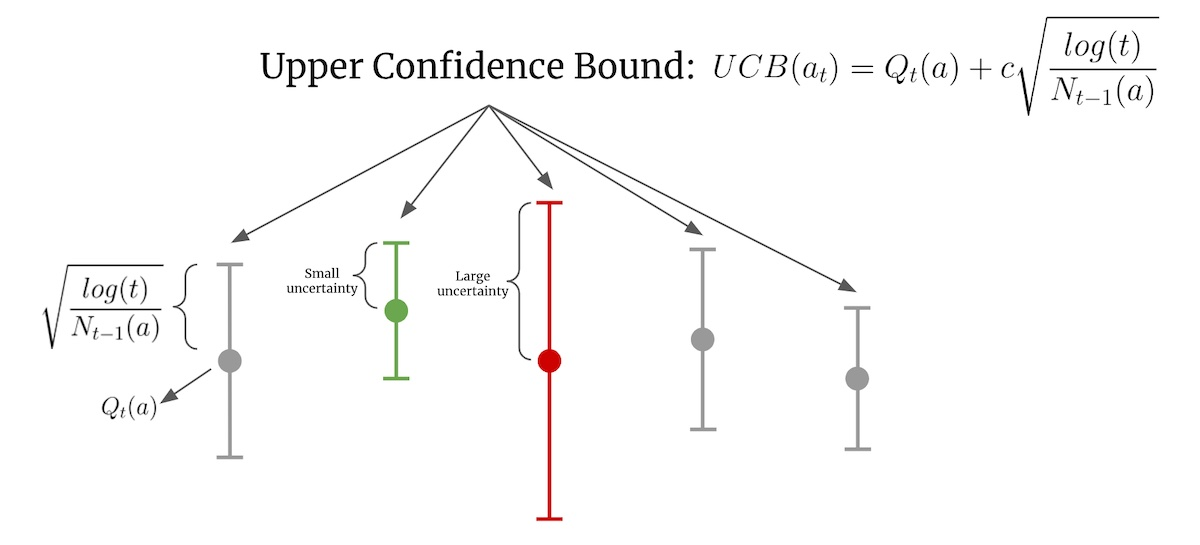
\includegraphics[width=\textwidth]{body_matter/bandits/images/ucb.jpg}
    \caption{Οπτικοποίηση \en{UCB} \cite{yan2022bandit} διάφορων χεριών}
    \label{fig:ucb}
\end{figure}

\subsection{Δειγματοληψία \en{Thompson}}

Η δειγματοληψία \en{Thompson} χτίζει μια κατανομή πιθανότητας βασισμένη σε ιστορικές ανταμοιβές και μετά δειγματοληπτεί από την κατανομή καθε δράσης για την επιλογή αυτής που επιφέρει την μέγιστη αναμενόμενη ανταμοιβή. Στην απλή περίπτωση που η ανταμοιβή είναι δυαδική (0 ή 1) και άρα θέλουμε να υπολογίσουμε την πιθανότητα να υπάρχει ανταμοιβή, χρησιμοποιειται η κατανομή Βήτα για την μοντελοποίηση των κατανομών των ανταμοιβών του κάθε χεριού. Η κατανομή Βήτα παίρνει δύο παραμέτρους, τα $α$ και $β$, όπου $α$ είναι οι φορές που η ανταμοιβή είναι 1 και $β$ είναι η φορές που η ανταμοιβή ήταν $0$. Η μέση τιμή της κατανομής είναι $\frac{α}{α+β}$, το οποίο αντιστοιχεί στο κλάσμα των επιτυχιών προς το σύνολο των προσπαθειών. Για την επιλογή μιας δράσης, δειγματοληπτούμε από την κατανομή Βήτα κάθε χεριού και επιλέγουμε τον χέρι με την υψηλότερη δειγματολημμένη τιμή \cite{thompsonsampling}.

H κατανομή Βήτα για διάφορα $α$ και $β$ φαίνεται στο Σχήμα~\ref{fig:beta_distribution}. Όσο αυξάνεται το πλήθων των $α$ και $β$, η κατανομή στενεύει και άρα βρίσκεται πιο κοντά στην πιθανότητα που έχει το κάθε χέρι να επιφέρει ανταμοιβή. Έτσι χέρια που έχουν δοκιμαστεί λιγότερο και έχουν πιο διευρυμένη κατανομή, έχουν πιθανότητες να δοκιμαστούν ως εξερεύνηση για να εξεταστεί αν επιφέρουν καλύτερες ανταμοιβές.

\begin{figure}
    \centering
    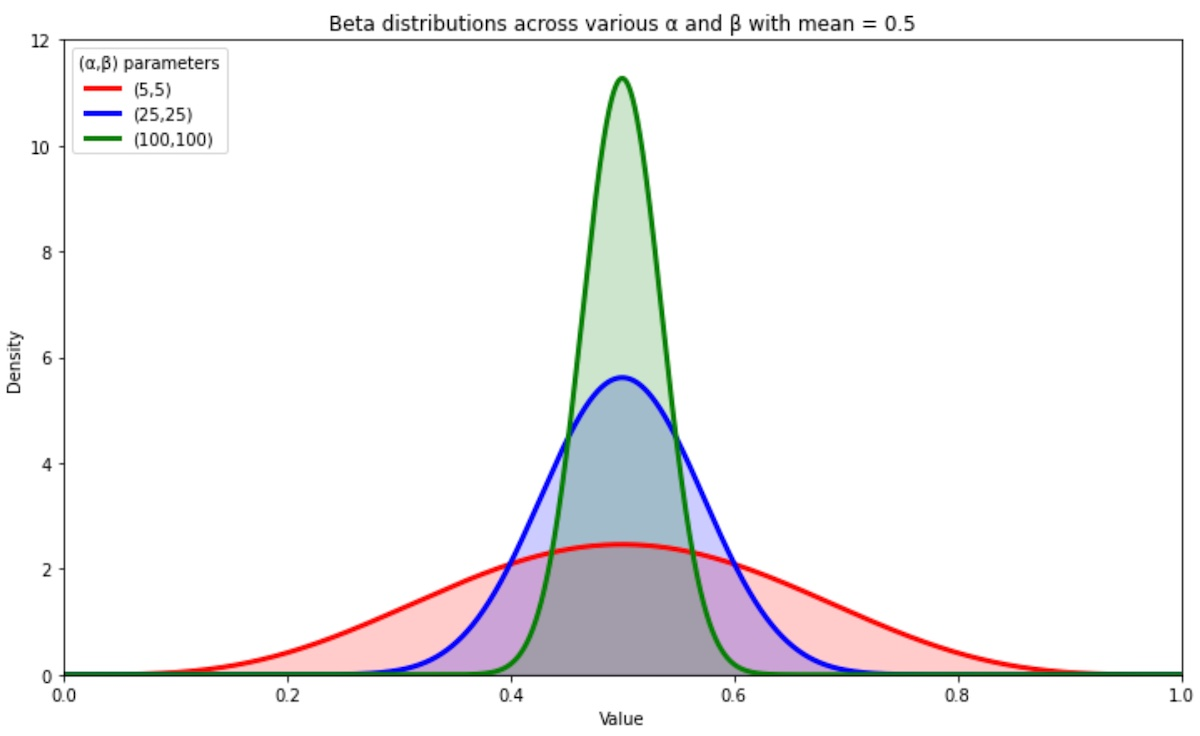
\includegraphics[width=\textwidth]{body_matter/bandits/images/beta-distribution.jpg}
    \caption{Η κατανομή Βήτα στενεύει όσο τα $α$ και $β$ μεγαλώνουν}
    \label{fig:beta_distribution}
\end{figure}

Η δειγματοληψία \en{Thompson} δουλεύει και σε περιπτώσεις που η ανταμοιβή δεν είναι δυαδική, απλά η κατανομή που χρησιμοποιειται δεν είναι η Βήτα, αλλά κάποια άλλη.

\subsection{Ο αλγόριθμος \en{EXP3}}

Το \en{EXP3} σημαίνει \en{Exponential-weight algorithm for Exploration and Exploitation}, δηλαδή Αλγόριθμος εκθετικών βαρών για αναζήτηση και εκμετάλλευση. Ο τρόπος που δουλεύει είναι διατηρώντας μια λίστα με τα βάρη κάθε δράσης και χρησιμοποιώντας τα για να επιλέξει τυχαία ποια δράση να κάνει μετά. Τέλος, τα αντίστοιχα βάρη αυξάνονται/μειώνονται όταν η ανταμοιβή είναι καλή/κακή. Επίσης υπάρχει ο παράγοντας $γ$, ο οποίος ορίζει την θέληση να επιλέξουμε μια δράση με ομοιόμορφη τυχαιότητα. Έτσι, αν $γ=1$, τα βάρη δεν έχουν καμία επίδραση στις επιλογές σε κάθε βήμα.

Ο αλγόριθμος μπορεί να περιγραφεί ως:
\begin{enumerate}
    \item Δοθέντος $γ \in [0,1]$, αρχικοποιούμε τα βάρη $w_i(1)=1$ για $ι = 1,\ldots,K$, όπου $K$ είναι τα χέρια.
    \item Για κάθε γύρο $t$:
          \begin{enumerate}
              \item Θέτουμε $p_i(t) = (1-γ)\frac{w_i(t)}{\sum_{j=1}^K w_j(t)} + \frac{γ}{K}$ για κάθε $i$.
              \item Επιλέγουμε την επόμενη δράση $i_t$ τυχαία με βάση την κατανομή του $p_i(t)$.
              \item Παρατηρούμε την ανταμοιβή $x_{i_t}(t)$.
              \item Ορίζουμε την αναμενόμενη ανταμοιβή $\hat{x}_{i_t}(t)$ να είναι $x_{i_t}(t)/p_{i_t}(t)$. Αυτό το βήμα εξασφαλίζει ότι η δεσμευμένη προσδοκία της αναμενόμενης ανταμοιβής είναι η πραγματική ανταμοιβή.
              \item Θέτουμε $w_{i_t}(t+1) = w_{i_t}(t)e^{γ\hat{x}_{i_t}(t)/K}$
              \item Θέτουμε όλα τα άλλα $w_j(t+1) = w_j(t)$.
          \end{enumerate}
\end{enumerate}

\section{\en{Contextual Bandits}}
Η περίπτωση \en{bandits} που μας ενδιαφέρει είναι αυτή στην οποία ο αλγόριθμος έχει πρόσβαση σε πληροφορίες σχετικά με το συγκείμενο του περιβάλλοντος, τις οποίες θα μπορούσε να χρησιμοποιήσει για να πάρει καλύτερες αποφάσεις. Το πρόβλημα και η μετρική (η μετάνοια) που μελετήσαμε νωρίτερα δεν χρησιμοποιούσαν τέτοια δεδομένα και προσπαθούσαν να επιλέξουν την καλύτερη κίνηση. Το πρόβλημα αυτό στην μορφή που περιγράφουμε εδώ, μελετήθηκε από τον \en{John Langford}  και τον \en{Tong Zhang} στο \cite{langford_epoch-greedy_2007}, καθώς σε προβλήματα στον πραγματικό κόσμο πάντα υπάρχουν επιπλέον πληροφορίες που μπορεί να χρησιμοποιήσει ο πράκτορας για να πάρει καλύτερες αποφάσεις. Συγκεκριμένα το πρόβλημα που προσπαθούσαν να λύσουν είναι η αντιστοίχηση διαφημισεων σε περιεχόμενο ιστοσελίδων στο ίντερνετ.

Για να μελετήσουμε αυτή την νέα περίπτωση θα χρειαστεί να επεκτείνουμε το πλαίσιο στο οποίο εργαζόμαστε, καθώς για τον ορισμό της μετάνοιας, ώστε μπορέσουμε να μοντελοποιήσουμε αυτα τα προβλήματα, τα οποία περιέχουν πληροφορίες συγκειμένου. Είναι σημαντικό να έχουμε υπ'όψιν ότι όταν σχεδιάζουμε μια καινούρια μετρική έχουμε να  συμβιβαστούμε μεταξύ της μεροληψίας και της διακύμανσης \en{bias-variance trade-off}. Μεροληψίας από την άποψη ότι δεν θέλουμε να βρούμε μια κακή μετρική με την οποία να συγκριθούμε, γιατί τότε κάθε αλγόριθμος που θα έχει παρόμοια απόδοση με την μετρική θα έχει κακή απόδοση. Από την άλλη, ο συναγωνισμός με μια καλύτερη μετρική μπορεί να είναι πολύ δύσκολος από την προοπτική της μάθησης και αυτή η τιμωρία μπορεί να υπερτερεί των πλεονεκτημάτων.

Αν προσεγγίσουμε τους \en{contextual bandits} με χρήση των ιδεών από τους ανταγωνιστικούς \en{bandits}, τότε το πρόβλημα παίρνει την παρακάτω μορφή:

\begin{enumerate}
    \item Ο αντίπαλος κρυφά διαλέγει ανταμοιβές $(x_t)_{t=1}^n$ με $x_t \in [0,1]^k$
    \item Ο αντίπαλος κρυφά διαλέγει συγκείμενο $(c_t)_{t=1}^n$ με $c_t \in \mathcal{C}$, όπου $\mathcal{C}$ είναι το σταθερό σύνολο των πιθανών συγκειμένων.
    \item Για τους γύρους $t=1,2,\ldots,n$:
          \begin{enumerate}
              \item Ο πράκτορας παρατηρεί συγκείμενο  $c_t \in \mathcal{C}$
              \item Ο πράκτορας διαλέγει κατανομή $P_t \in \mathcal{P}_{k-1}$ και παίρνει δείγμα $A_t$  από το $P_t$
              \item Ο πράκτορας παρατηρεί ανταμοιβή $X_t = x_{tA_t}$
          \end{enumerate}
\end{enumerate}

Το πλαίσιο των \en{contextual bandits} μας προσφέρει το εργαλείο για να περιγράψουμε το πρόβλημα των συστάσεων που θέλουμε να λύσουμε. Μετά την εισαγωγή του προβλήματος σαν μέθοδο για την επίλυση τέτοιου είδους προβλημάτων το 2007, έχει υπάρξει σημαντική έρευνα, αλλά και χρήση στην βιομηχανία τέτοιων μεθόδων, ειδικά σε περιπτώσεις που το πλήθος των αντικειμένων αλλάζει δυναμικά, πχ νέα άρθρα προστίθενται κάθε μέρα, ενώ τα παλιά άρθρα είναι πλεον λιγότερο σημαντικά. Έτσι εταιρίες όπως η \en{Microsoft}, το \en{LinkedIn}, το \en{Netflix} και άλλες χρησιμοποιούν τέτοιες μεθόδους για να προτείνουν άρθρα, διαφημίσεις ή ταινίες αντίστοιχα. Το \en{Netflix} χρησιμοποιεί επίσης \en{contextual bandits} για να επιλέξει την εικόνα που δείχνει για κάθε ταινία \cite{blog_artwork_2017}.  Στα επόμενα μέρη της διπλωματικής, δεν αναλύσουμε περισσότερο τις ιδιότητες των αλγορίθμων αυτών, ουτε θα προχωρήσουμε σε αναλύσεις της μετάνοιας τους, αλλά θα τους χρησιμοποιήσουμε μόνο βάση της ανάλυσης στις εργασίες που εισήχθηκαν.

